\chapter{Kiểm định và đánh giá kết quả}
Chương này chúng tôi trình bày kết quả sử dụng ứng dụng webfuzzer để kiểm thử một số ứng dụng web và so sánh trực tiếp với quá trình kiểm thử bằng chức năng \texttt{Intruder} của công cụ Burp Suite để đánh giá kết quả đạt được thông qua quá trình thiêt kế và hiện thực ứng dụng.
\section{Thiết lập kiểm thử ở Burp Suite}
Ở ứng dụng Burp Suite, chúng tôi cần thiết lập thời gian timeout của các \acrshort{http} request kiểm thử, danh sách payload và các chuỗi, biểu thức chính quy so trùng trên response. Các thông số trên lần lượt tương ứng với các trường \texttt{time}, \texttt{payloadFile} và \texttt{match, matchFile, regex} trong cấu hình kiểm thử. Chức năng \texttt{Intruder} không cho phép điều chỉnh timeout riêng của các request trong chức năng này, chúng tôi phải thiết lập thời gian timeout toàn cục cho một dự án (project) của Burp Suite dưới dạng đối tượng JSON như Đoạn mã \ref{lst:setup-timeout-burp} sau. Đây cũng là một sự tiện lợi khi sử dụng webfuzzer vì người dùng có thể dễ dàng điều chỉnh thông số này ở cấu hình kiểm thử tùy theo từng loại lỗ hổng.
\begin{lstlisting}[style=ES6, label={lst:setup-timeout-burp}, caption={Thiết lập thời gian timeout của request kiểm thử ở Burp Suite}]
"timeouts":{
    "domain_name_resolution_timeout":300000,
    "failed_domain_name_resolution_timeout":60000,
    "normal_timeout":10000,
    "open_ended_response_timeout":10000
},
Các chuỗi và biểu thức chính quy so trùng có thể được thêm vào bằng tay ở mục \texttt{Grep - Match} trong tab \texttt{Options} như Hình \ref{fig:setup-grep-string-regex} sau.
\begin{figure}[H]
    \centering
        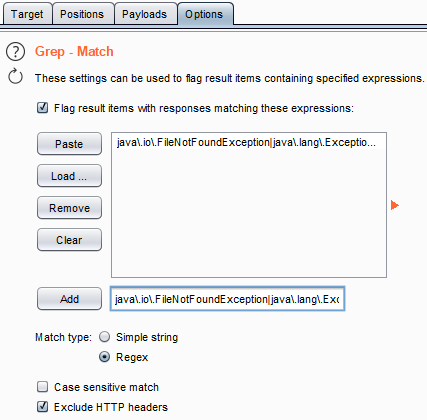
\includegraphics[width=0.6\textwidth,keepaspectratio=true]{images/setup-grep-string-regex.png}
    \caption{Thêm thiết lập so trùng vào cấu hình kiểm thử ở Burp Suite}
    \label{fig:setup-grep-string-regex}
\end{figure}
Tương tự, chức năng danh sách payload có thể được thêm vào tuần tự hoặc trích xuất từ tập tin ở mục \texttt{Payload Options [Simple list]} trong tab \texttt{Payloads} như Hình \ref{fig:setup-payload-list} sau. Việc lưu trữ và sao chép các thiết lập kiểm thử (payload, các chuỗi so trùng) giữa các đối tượng trong chức năng \texttt{Intruder} khá phiền phức so với webfuzzer. Người dùng webfuzzer chỉ việc chọn những cấu hình kiểm thử thường dùng đã được định nghĩa sẵn ở backend, đây cũng là một ưu điểm của ứng dụng so với Burp Suite.
\begin{figure}[H]
    \centering
        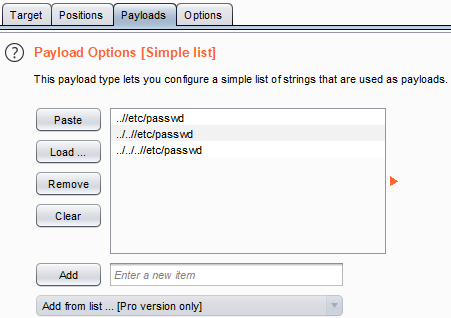
\includegraphics[width=0.6\textwidth,keepaspectratio=true]{images/setup-payload-list.png}
    \caption{Thêm payload vào cấu hình kiểm thử ở Burp Suite}
    \label{fig:setup-payload-list}
\end{figure}
Trong quá trình kiểm thử bằng Burp Suite, chúng tôi phải tự nhận diện lỗ hổng thủ công thông qua giao diện kiểm thử của chức năng \texttt{Intruder} như Hình \ref{fig:fuzzing-burp} sau.
\begin{figure}[H]
    \centering
        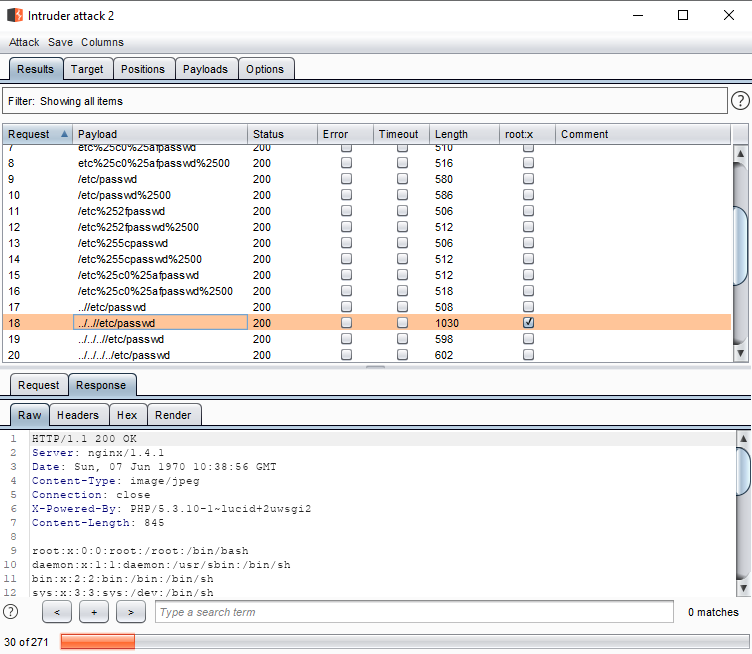
\includegraphics[width=\textwidth,keepaspectratio=true]{images/fuzzing-burp.png}
    \caption{Giao diện kiểm thử bằng chức năng \texttt{Intruder} của Burp Suite}
    \label{fig:fuzzing-burp}
\end{figure}
Từng request kiểm thử chứa payload tương ứng sẽ được hiển thị thành một dòng trên giao diện, lần lượt thể hiện các thông tin của request đó, backend của webfuzzer cũng xuất ra kết quả kiểm thử tương tự trên terminal. Các chuỗi và biểu thức chính quy so trùng được hiển thị dưới dạng một cột, cột này sẽ được đánh dấu khi nội dung response tương ứng có chứa chuỗi đó như Hình \ref{fig:fuzzing-burp}. Khung bên dưới hiển thị nội dung chi tiết của response ứng với request kiểm thử đang chọn ở trên. Tương tự khi request kiểm thử vượt quá thời gian timeout đã thiết lập thì cột \texttt{Timeout} trên giao diện sẽ được đánh dấu. Sau khi quá trình kiểm thử kết thúc, người dùng phải tự hệ thống lại xem payload nào phát hiện được lỗ hổng.\par
\end{lstlisting}
\section{Tập kiểm thử và kết quả đánh giá công cụ}
Để quá trình đánh giá kết quả được khách quan, chúng tôi sử dụng tập kiểm thử gồm có các trang web có và không có các lỗ hổng \acrshort{lfi} và time-based \acrshort{sqli}. Chúng tôi đồng thời kiểm thử các trang web này bằng webfuzzer và Burp Suite, so sánh kết quả kiểm thử, các payload phát hiện lỗ hổng nếu có, và thời gian kiểm thử mỗi mục tiêu của hai phần mềm này. Máy tính thực hiện kiểm thử trên cả hai phần mềm sử dụng CPU Intel Core i5-9400F và 8GB DDR4 RAM, trên hệ điều hành Ubuntu 20.04 LTS Focal. Ở chức năng \texttt{Intruder} của Burp Suite chúng tôi thiết lập số lượng luồng (threads) là 1, số lần thử gửi lại request khi thất bại là 0, và không áp dụng các phương pháp encode nào khác trên payload vì trong webfuzzer chúng tôi không hiện thực các chức năng này. Trong quá trình trình bày kết quả đánh giá, chúng tôi rút gọn trường cookies và headers của các đối tượng kiểm thử (request mẫu) trong trường hợp không cần thiết. Chúng tôi ghi lại kết quả đánh giá dưới dạng Bảng \ref{tab:sample-testing-results} sau, trong đó \texttt{N} là số payload phát hiện lỗi và \texttt{T} là thời gian kiểm thử của ứng dụng tính bằng mili giây.
\FloatBarrier
\begin{table}[ht]
    \centering
    \caption{Mẫu bảng so sánh kết quả kiểm thử ứng dụng webfuzzer so với Burp Suite}
    \label{tab:sample-testing-results}
    \begin{tabular}[ht]{ccccc}
        \toprule[1pt]\midrule[0.3pt]
            \multirow{2}{*}{\textbf{Loại lỗ hổng}}&\multicolumn{2}{c}{\textbf{Webfuzzer}}&\multicolumn{2}{c}{\textbf{Burp Suite}}\\
            \cmidrule(lr){2-3}\cmidrule(lr){4-5}{}&Số payload&Thời gian&Số payload&Thời gian\\
        \midrule[0.3pt]
            \textbf{\acrshort{lfi}}&N&T&N&T\\\addlinespace
            \textbf{Time-based \acrshort{sqli}}&N&T&N&T\\
        \midrule[0.3pt]\bottomrule[1pt]
    \end{tabular}
\end{table}
\FloatBarrier
Nội dung request mẫu và kết quả kiểm thử các request này trên hai ứng dụng lần lượt được trình bày bằng các Đoạn mã và các Bảng dưới đây.
\begin{lstlisting}[style=ES6, label={lst:base-request-1}, caption={Request mẫu 1 có lỗ hổng \acrshort{lfi}}]
{
    "url": "http://testphp.vulnweb.com:80/showimage.php?file=§./pictures/1.jpg§",
    "cookies": "",
    "headers": { ... },
    "method": "get"
}
\end{lstlisting}
\FloatBarrier
\begin{table}[ht]
    \centering
    \caption{Kết quả kiểm thử request mẫu 1}
    \label{tab:testing-result-1}
    \begin{tabular}[ht]{ccccc}
        \toprule[1pt]\midrule[0.3pt]
            \multirow{2}{*}{\textbf{Loại lỗ hổng}}&\multicolumn{2}{c}{\textbf{Webfuzzer}}&\multicolumn{2}{c}{\textbf{Burp Suite}}\\
            \cmidrule(lr){2-3}\cmidrule(lr){4-5}{}&Số payload&Thời gian&Số payload&Thời gian\\
        \midrule[0.3pt]
            \textbf{\acrshort{lfi}}&1&89998&1&88400\\
        \midrule[0.3pt]\bottomrule[1pt]
    \end{tabular}
\end{table}
\FloatBarrier
\begin{lstlisting}[style=ES6, label={lst:base-request-2}, caption={Request mẫu 2 có lỗ hổng time-based \acrshort{sqli}}]
{
    "url": "http://testphp.vulnweb.com:80/search.php?test=query",
    "cookies": "",
    "headers": { ... },
    "data": {
        "searchFor": "a§§",
        "goButton": "go"
    },
    "method": "post"
}
\end{lstlisting}
\FloatBarrier
\begin{table}[ht]
    \centering
    \caption{Kết quả kiểm thử request mẫu 2}
    \label{tab:testing-result-2}
    \begin{tabular}[ht]{ccccc}
        \toprule[1pt]\midrule[0.3pt]
            \multirow{2}{*}{\textbf{Loại lỗ hổng}}&\multicolumn{2}{c}{\textbf{Webfuzzer}}&\multicolumn{2}{c}{\textbf{Burp Suite}}\\
            \cmidrule(lr){2-3}\cmidrule(lr){4-5}{}&Số payload&Thời gian&Số payload&Thời gian\\
        \midrule[0.3pt]
            \textbf{Time-based \acrshort{sqli}}&14&298195&14&299600\\
        \midrule[0.3pt]\bottomrule[1pt]
    \end{tabular}
\end{table}
\FloatBarrier
\begin{lstlisting}[style=ES6, label={lst:base-request-3}, caption={Request mẫu 3}]
{
    "url": "http://www.daotaonlyt.edu.vn:80/img/§§",
    "cookies": { ... },
    "headers": { ... },
    "method": "get"
}
\end{lstlisting}
\FloatBarrier
\begin{table}[ht]
    \centering
    \caption{Kết quả kiểm thử request mẫu 3}
    \label{tab:testing-result-3}
    \begin{tabular}[ht]{ccccc}
        \toprule[1pt]\midrule[0.3pt]
            \multirow{2}{*}{\textbf{Loại lỗ hổng}}&\multicolumn{2}{c}{\textbf{Webfuzzer}}&\multicolumn{2}{c}{\textbf{Burp Suite}}\\
            \cmidrule(lr){2-3}\cmidrule(lr){4-5}{}&Số payload&Thời gian&Số payload&Thời gian\\
        \midrule[0.3pt]
            \textbf{\acrshort{lfi}}&0&2925&0&3500\\
        \midrule[0.3pt]\bottomrule[1pt]
    \end{tabular}
\end{table}
\FloatBarrier
\begin{lstlisting}[style=ES6, label={lst:base-request-4}, caption={Request mẫu 4 có lỗ hổng time-based \acrshort{sqli}}]
{
    "url": "http://artistclub.vn:80/",
    "cookies": { ... },
    "headers": { ... },
    "data": {
        "email_nhantin": "aaaa@gmail.com§§"
    },
    "method": "post"
}
\end{lstlisting}
\FloatBarrier
\begin{table}[ht]
    \centering
    \caption{Kết quả kiểm thử request mẫu 4}
    \label{tab:testing-result-4}
    \begin{tabular}[ht]{ccccc}
        \toprule[1pt]\midrule[0.3pt]
            \multirow{2}{*}{\textbf{Loại lỗ hổng}}&\multicolumn{2}{c}{\textbf{Webfuzzer}}&\multicolumn{2}{c}{\textbf{Burp Suite}}\\
            \cmidrule(lr){2-3}\cmidrule(lr){4-5}{}&Số payload&Thời gian&Số payload&Thời gian\\
        \midrule[0.3pt]
            \textbf{Time-based \acrshort{sqli}}&7&92952&7&89700\\
        \midrule[0.3pt]\bottomrule[1pt]
    \end{tabular}
\end{table}
\FloatBarrier
\begin{lstlisting}[style=ES6, label={lst:base-request-5}, caption={Request mẫu 5}]
{
    "url": "http://artistclub.vn:80/upload/sanpham/
        §b814bf98-5aad-4146-ade5-6a41f3b631490060_323x360.jpeg§",
    "cookies": { ... },
    "headers": { ... },
    "method": "get"
}
\end{lstlisting}
\FloatBarrier
\begin{table}[ht]
    \centering
    \caption{Kết quả kiểm thử request mẫu 5}
    \label{tab:testing-result-5}
    \begin{tabular}[ht]{ccccc}
        \toprule[1pt]\midrule[0.3pt]
            \multirow{2}{*}{\textbf{Loại lỗ hổng}}&\multicolumn{2}{c}{\textbf{Webfuzzer}}&\multicolumn{2}{c}{\textbf{Burp Suite}}\\
            \cmidrule(lr){2-3}\cmidrule(lr){4-5}{}&Số payload&Thời gian&Số payload&Thời gian\\
        \midrule[0.3pt]
            \textbf{\acrshort{lfi}}&0&4086&0&4900\\
        \midrule[0.3pt]\bottomrule[1pt]
    \end{tabular}
\end{table}
\FloatBarrier
\begin{lstlisting}[style=ES6, label={lst:base-request-6}, caption={Request mẫu 6}]
{
    "url": "http://mwc.com.vn:80/search?s=a§§",
    "cookies": { ... },
    "headers": { ... },
    "method": "get"
}
\end{lstlisting}
\FloatBarrier
\begin{table}[ht]
    \centering
    \caption{Kết quả kiểm thử request mẫu 6}
    \label{tab:testing-result-6}
    \begin{tabular}[ht]{ccccc}
        \toprule[1pt]\midrule[0.3pt]
            \multirow{2}{*}{\textbf{Loại lỗ hổng}}&\multicolumn{2}{c}{\textbf{Webfuzzer}}&\multicolumn{2}{c}{\textbf{Burp Suite}}\\
            \cmidrule(lr){2-3}\cmidrule(lr){4-5}{}&Số payload&Thời gian&Số payload&Thời gian\\
        \midrule[0.3pt]
            \textbf{Time-based \acrshort{sqli}}&0&52760&0&54300\\
        \midrule[0.3pt]\bottomrule[1pt]
    \end{tabular}
\end{table}
\FloatBarrier
\begin{lstlisting}[style=ES6, label={lst:base-request-7}, caption={Request mẫu 7 có lỗ hổng time-based \acrshort{sqli}}]
{
    "url": "http://www.monitoringris.org:80/index.php?id=30§§",
    "cookies": "",
    "headers": { ... },
    "method": "get"
}
\end{lstlisting}
\FloatBarrier
\begin{table}[ht]
    \centering
    \caption{Kết quả kiểm thử request mẫu 7}
    \label{tab:testing-result-7}
    \begin{tabular}[ht]{ccccc}
        \toprule[1pt]\midrule[0.3pt]
            \multirow{2}{*}{\textbf{Loại lỗ hổng}}&\multicolumn{2}{c}{\textbf{Webfuzzer}}&\multicolumn{2}{c}{\textbf{Burp Suite}}\\
            \cmidrule(lr){2-3}\cmidrule(lr){4-5}{}&Số payload&Thời gian&Số payload&Thời gian\\
        \midrule[0.3pt]
            \textbf{Time-based \acrshort{sqli}}&4&434913&4&430200\\
        \midrule[0.3pt]\bottomrule[1pt]
    \end{tabular}
\end{table}
\FloatBarrier
\begin{lstlisting}[style=ES6, label={lst:base-request-8}, caption={Request mẫu 8 có lỗ hổng time-based \acrshort{sqli}}]
{
    "url": "http://www.daotaonlyt.edu.vn:80/index.php?id=320§§",
    "cookies": { ... },
    "headers": { ... },
    "method": "get"
}
\end{lstlisting}
\FloatBarrier
\begin{table}[ht]
    \centering
    \caption{Kết quả kiểm thử request mẫu 8}
    \label{tab:testing-result-8}
    \begin{tabular}[ht]{ccccc}
        \toprule[1pt]\midrule[0.3pt]
            \multirow{2}{*}{\textbf{Loại lỗ hổng}}&\multicolumn{2}{c}{\textbf{Webfuzzer}}&\multicolumn{2}{c}{\textbf{Burp Suite}}\\
            \cmidrule(lr){2-3}\cmidrule(lr){4-5}{}&Số payload&Thời gian&Số payload&Thời gian\\
        \midrule[0.3pt]
            \textbf{Time-based \acrshort{sqli}}&4&66493&4&64900\\
        \midrule[0.3pt]\bottomrule[1pt]
    \end{tabular}
\end{table}
\FloatBarrier
\begin{lstlisting}[style=ES6, label={lst:base-request-9}, caption={Request mẫu 9 có lỗ hổng time-based \acrshort{sqli}}]
{
    "url": "http://csdl.vietnamtourism.gov.vn:80/index.php/
        search/?data=cslt&title=a§§",
    "cookies": "",
    "headers": { ... },
    "method": "get"
}
\end{lstlisting}
\FloatBarrier
\begin{table}[ht]
    \centering
    \caption{Kết quả kiểm thử request mẫu 9}
    \label{tab:testing-result-9}
    \begin{tabular}[ht]{ccccc}
        \toprule[1pt]\midrule[0.3pt]
            \multirow{2}{*}{\textbf{Loại lỗ hổng}}&\multicolumn{2}{c}{\textbf{Webfuzzer}}&\multicolumn{2}{c}{\textbf{Burp Suite}}\\
            \cmidrule(lr){2-3}\cmidrule(lr){4-5}{}&Số payload&Thời gian&Số payload&Thời gian\\
        \midrule[0.3pt]
            \textbf{Time-based \acrshort{sqli}}&86&1572156&86&1481300\\
        \midrule[0.3pt]\bottomrule[1pt]
    \end{tabular}
\end{table}
\FloatBarrier
\begin{lstlisting}[style=ES6, label={lst:base-request-10}, caption={Request mẫu 10 có lỗ hổng time-based \acrshort{sqli}}]
{
    "url": "http://www.hanglahangdoc.com:80/tim_kiem.aspx?keyword=a§§",
    "cookies": { ... },
    "headers": { ... },
    "method": "get"
}
\end{lstlisting}
\FloatBarrier
\begin{table}[ht]
    \centering
    \caption{Kết quả kiểm thử request mẫu 10}
    \label{tab:testing-result-10}
    \begin{tabular}[ht]{ccccc}
        \toprule[1pt]\midrule[0.3pt]
            \multirow{2}{*}{\textbf{Loại lỗ hổng}}&\multicolumn{2}{c}{\textbf{Webfuzzer}}&\multicolumn{2}{c}{\textbf{Burp Suite}}\\
            \cmidrule(lr){2-3}\cmidrule(lr){4-5}{}&Số payload&Thời gian&Số payload&Thời gian\\
        \midrule[0.3pt]
            \textbf{Time-based \acrshort{sqli}}&6&219560&6&212800\\
        \midrule[0.3pt]\bottomrule[1pt]
    \end{tabular}
\end{table}
\FloatBarrier
Qua quá trình kiểm thử các request mẫu trên, chúng tôi nhận thấy các payload phát hiện lỗi ở cả hai ứng dụng đều giống hệt nhau, đây là thành công lớn nhất trong quá trình hiện thực webfuzzer, ứng dụng này đã mô phỏng thành công một phần chức năng \texttt{Intruder} của Burp Suite như hướng phát triển công cụ đã đề ra ở \textbf{Chương 4}. Thời gian kiểm thử của webfuzzer cũng xấp xỉ Burp Suite, chỉ chậm hơn khoảng 2-10 giây tùy vào mỗi request mẫu, hơn nữa webfuzzer có phần nhanh hơn Burp Suite ở các request mẫu mà cả hai ứng dụng đều không phát hiện được lỗ hổng. Vì vậy ngoài lý do không thể tránh khỏi về kết nối, đường truyền giữa các lần kiểm thử, chúng tôi nhận định khoảng thời gian chênh lệch trong việc kiểm thử các request mẫu có lỗ hổng phần lớn đến từ việc lưu trữ kết quả kiểm thử vào cơ sở dữ liệu, do đó chênh lệch thời gian vài giây là một khoản đánh đổi chấp nhận được. Trong quá trình sử dụng ứng dụng, chúng tôi nhận thấy giao diện người dùng tương đối mượt mà, thân thiện với người dùng hơn BurpSuite. Thời gian phản hồi của các \acrshort{http} request gửi đến backend webfuzzer được triển khai ở máy chủ nội bộ (\href{http://localhost:13336/}{\texttt{http://localhost:13336/}}) hoặc ở \acrshort{vps} (\href{http://61.28.235.183:13336/}{\texttt{http://61.28.235.183:13336/}}) chỉ dao động trong khoảng 20-200 mili giây.\par
Xét về trải nghiệm người dùng, ứng dụng webfuzzer trực quan và tiện lợi hơn Burp Suite rất nhiều. Thay vì việc thiết lập cấu hình kiểm thử và nhận diện lỗ hổng thủ công ở Burp Suite như đã mô tả ở \textbf{Đề mục 7.1}, webfuzzer đã tích hợp sẵn khả năng nhận diện lỗ hổng trong mô-đun kiểm thử, đồng thời tổng hợp sẵn những cấu hình kiểm thử tiện dụng, dễ dàng chỉnh sửa. Người dùng chỉ việc chọn request mẫu và loại lỗ hổng, kết quả kiểm thử sẽ được ứng dụng webfuzzer cung cấp chi tiết, request kiểm thử chứa payload nào bị timeout, hay trả về response có chứa chuỗi so trùng nào, phát hiện được lỗ hổng gì. Tổng kết từ các nhận định trên, chúng tôi đánh giá ứng dụng webfuzzer đã được hiện thực hoàn chỉnh ở mức chấp nhận được, thỏa mãn yêu cầu thiết kế hệ thống.